\newpage

\subsection*{Question 4}

\noindent [10 pts] Consider the regular grammar $G_1 = (V_1, \Sigma, S_1, P_1)$, where $V_1 = \{S_1, A, B\}$,
$\Sigma = \{a, b\}$, and $P_1$ consists of the productions $S_1 \rightarrow abA$, $A \rightarrow baB$, and 
$B \rightarrow aA | bb$. Also consider the grammar $G_2 = (\{S_2, B\}, \Sigma, S_2, P_2)$, where the productions
in $P_2$ are:
\begin{align*}
    S_2 &\rightarrow aaB | \lambda\\
    B &\rightarrow bB | ab
\end{align*}
\noindent Give a left linear grammar for the language $L(G_1) \cup L(G_2)$.

\subsection*{Answer}

\noindent First, let's find finite automaton that corresponds to the regular languages described by the regular grammars $G_1$ and $G_2$:\\
For $G_1$ we have:
\begin{center}
    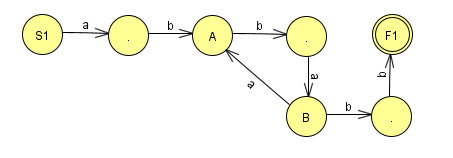
\includegraphics[width=0.5\textwidth]{img/graph9.png}
\end{center}
\noindent We inverse all the edges and swap the initial and final state:
\begin{center}
    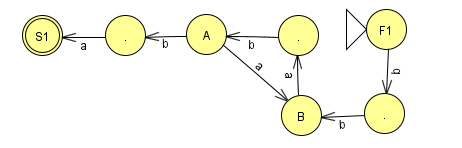
\includegraphics[width=0.5\textwidth]{img/graph10.png}
\end{center}
\noindent We now have the following grammar:
\begin{align*}
    F1 &\rightarrow bbB\\
    B &\rightarrow abA\\
    A &\rightarrow aB | ba
\end{align*}
\noindent We inverse the symbols to obtain the following left-linear grammar:
\begin{align*}
    F1 &\rightarrow Bbb\\
    B &\rightarrow Aba\\
    A &\rightarrow Ba | ab
\end{align*}
\newpage
\noindent We repeat the same process for $G_2$:\\ Finite automaton for $G_2$:
\begin{center}
    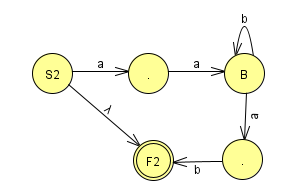
\includegraphics[width=0.35\textwidth]{img/graph11.png}
\end{center}
\noindent We inverse all the edges and swap the initial and final state:
\begin{center}
    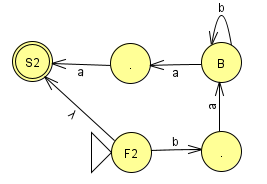
\includegraphics[width=0.35\textwidth]{img/graph12.png}
\end{center}
\noindent We now have the following grammar:
\begin{align*}
    F2 &\rightarrow baB | \lambda\\
    B &\rightarrow bB | aa
\end{align*}
\noindent We inverse the symbols to obtain the following left-linear grammar:
\begin{align*}
    F2 &\rightarrow Bab | \lambda\\
    B &\rightarrow Bb | aa
\end{align*}
\noindent We finally have to find the union of the found left-linear grammars. Let's call the new grammar $G$.We rename the non-terminals such that:\\
left-linear $G_1$:
\begin{align*}
    F1 &\rightarrow B_1bb\\
    B_1 &\rightarrow A_1ba\\
    A_1 &\rightarrow B_1a | ab
\end{align*}
\noindent And left-linear $G_2$:
\begin{align*}
    F2 &\rightarrow B_2ab | \lambda\\
    B_2 &\rightarrow B_2b | aa
\end{align*}

\noindent The left-linear grammar $G$ resulting from the union of left-linear $G_1$ and left-linear $G_2$:
\begin{align*}
    S &\rightarrow F1|F2\\
    F1 &\rightarrow B_1bb\\
    B_1 &\rightarrow A_1ba\\
    A_1 &\rightarrow B_1a | ab\\
    F2 &\rightarrow B_2ab | \lambda\\
    B_2 &\rightarrow B_2b | aa
\end{align*}




